\documentclass{scrartcl}
\usepackage[a4paper,left=3cm,right=3cm,top=3cm,bottom=3cm]{geometry}

\usepackage[utf8]{inputenc}
\usepackage[T1]{fontenc}
\usepackage{lmodern}
\usepackage[ngerman]{babel}
\usepackage{amsmath}
\usepackage{caption}
\usepackage{graphicx}
\usepackage{subfig}
\usepackage{hyperref}
\usepackage{listings}
\usepackage{listings}
\usepackage{color}

\definecolor{codegreen}{rgb}{0,0.6,0}
\definecolor{codegray}{rgb}{0.5,0.5,0.5}
\definecolor{codepurple}{rgb}{0.58,0,0.82}
\definecolor{codered}{rgb}{0.8, 0.2, 0.2}
\definecolor{backcolour}{rgb}{0.95,0.95,0.96}

\lstdefinelanguage{JavaScript}{
  keywords={typeof, new, true, false, catch, function, return, null, try, catch, switch, const, var, if, in, while, do, else, case, break},
  keywordstyle=\color{blue}\bfseries,
  ndkeywords={class, export, boolean, throw, implements, import, this},
  ndkeywordstyle=\color{codegray}\bfseries,
  identifierstyle=\color{black},
  sensitive=false,
  comment=[l]{//},
  morecomment=[s]{/*}{*/},
  commentstyle=\color{codepurple}\ttfamily,
  stringstyle=\color{codered}\ttfamily,
  morestring=[b]',
  morestring=[b]"
}
\lstdefinestyle{normal}{
    backgroundcolor=\color{backcolour},   
    commentstyle=\color{codegreen},
    keywordstyle=\color{magenta},
    numberstyle=\tiny\color{codegray},
    stringstyle=\color{codepurple},
    basicstyle=\ttfamily\footnotesize,
    breakatwhitespace=false,         
    breaklines=true,                 
    captionpos=b,                    
    keepspaces=true,                 
    numbers=left,                    
    numbersep=5pt,                  
    showspaces=false,                
    showstringspaces=false,
    showtabs=false,                  
    tabsize=2
}

\lstset{style=normal}

\hypersetup{
    colorlinks,
    citecolor=black,
    filecolor=black,
    linkcolor=black,
    urlcolor=black
}

\begin{document}
%%% Deckblatt
\begin{center}
    \thispagestyle{empty}
    \textbf{Berufsschule für Informationstechnik}

    Am Beruflichen Schulzentrum für Elektrotechnik

    Strehlener Platz 2, 01219 Dresden
    
    \vfill 
        \LARGE{\textbf{Ablaufdokumentation}}
        \linebreak
        
        \large{Version 1.0}
        \linebreak
        \linebreak

        \large{IT20/2}
        \linebreak
        \large{Lernfeld 9}
        \linebreak
        \linebreak

        \large{Paul Görtler}
        
        \large{Vincent Jablonski}  

        \large{Marcus Böhme}  
        \linebreak

        \large \today
    \vfill    
\end{center}
\newpage
\setcounter{page}{1}
%%% Deckblatt

\tableofcontents
\newpage

\begin{flushleft}
    \section{Firewall}
    \subsection{Server aufsetzen}
    Für das im Projekt benötigte Firewall-System wird die Open-Source Software Lösung IPFire verwendet. 

    \subsection{Konfiguration}
    Die IPFire VM verwendet folgendes Netzwerkkonfigurationsschema. \newline
    \textbf{GREEN + RED + ORANGE}. \newline

    Hierbei steht \textbf{GREEN} für das lokale Netzwerk, \textbf{RED} steht für das Internet und \textbf{ORANGE} für die DMZ. \newline \newline

    Dem Projektziel entsprechen verwendet die IPFire VM drei Network Adapter.
    Jeweils eine Adapter sorgt für eine Konnektivität in jedes der drei Netzwerke. \newline
    
    Folgende Konfigurationen werden verwendet.
    \begin{itemize}
        \item Network Adapter 1:
        \subitem \textbf{VMnet1:} 00:0C:29:01:9E:DA $\rightarrow$ $"$grünes Netzwerk"
        \item Network Adapter 2:
        \subitem \textbf{VMnet2:} 00:50:56:22:2C:E0 $\rightarrow$ $"$oranges Netzwerk"
        \item Network Adapter 3:
        \subitem \textbf{VMnet8:} 00:50:56:3F:82:8B $\rightarrow$ $"$rotes Netzwerk"
    \end{itemize}
    \ \newline

    \textbf{Folgende IPFire Firewall-Regeln wurden im Webinterface ergänzt.}
    
    \captionof{figure}{Firewall-Regeln}
    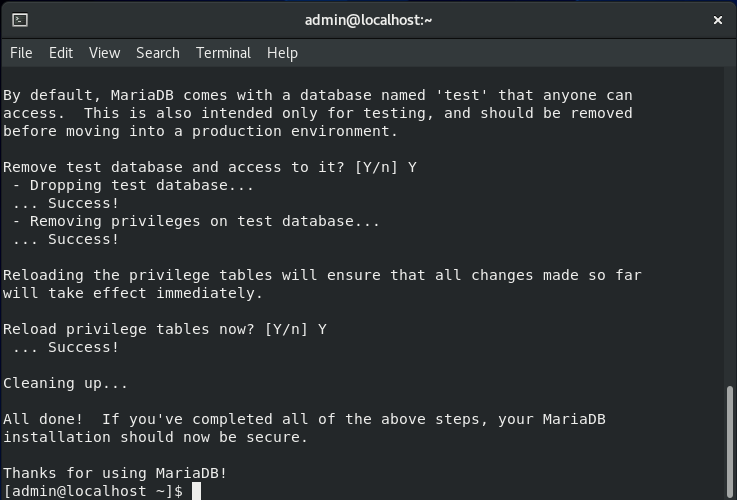
\includegraphics[width=\linewidth]{img/ipfire/6.png}
           
    \newpage

    \section{DNS und DHCP}
    \subsection{Server aufsetzen}
    Für eine sinnvolle Verwendung der Dienste DNS und DHCP wird ein eigenes System verwendet. Das System läuft auf einer CentOS 8 Version, welche direkt für die Nutzung im Serverbereich angepasst ist. Für die Umsetzung von DNS und DHCP wird die Software Lösung DNSMASQ verwendet.

    \subsection{Konfiguration}
    Für die Installation von DNSMASQ muss folgender Befehl ausgeführt werden.
    \begin{lstlisting}
        $ yum install dnsmasq\end{lstlisting}
    \ \newline
    Als Nächstes muss die Konfiguration von DNSMASQ angepasst werden.
    \begin{lstlisting}
        $ cp /etc/dnsmasq.conf /etc/dnsmasq.conf.orig
        $ nano /etc/dnsmasq.conf\end{lstlisting}
    \ \newline
    Folgende Einstellungen wurden eingetragen.
    \begin{lstlisting}
        interface=ens160
        listen-adress=127.0.0.1
        resolv-file=/etc/resolv.dnsmasq
        domain=Doubtful-Joy09.de
        dhcp-range=192.168.19.50,192.168.19.150,12h
        dhcp-leasefile=/var/lib/dnsmasq/dnsmasq.leases
        server=8.8.8.8\end{lstlisting}
    \ \newline
    Die Services müssen für die lokale Firewall des DNS und DHCP Servers freigegeben werden.
    \begin{lstlisting}
        $ firewall-cmd --zone=public --add-service=dns --permanent
        $ firewall-cmd --zone=public --add-service=dhcp --permanent
        $ firewall-cmd --reload\end{lstlisting}
    \ \newline
    Um DNS-Einträge hinzuzufügen, muss die hosts\textit{($"$/etc/hosts")} Datei bearbeitet werden.
    \begin{lstlisting}
    192.168.19.3 ipfire.Doubtful-Joy09.de
    192.168.242.4 ticketsystem.Doubtful-Joy09.de\end{lstlisting}

    \newpage

    \section{Datenbank}
    \subsection{Server aufsetzen}
    Für eine sinnvolle Verwendung der Dienste DNS und DHCP wird ein eigenes System verwendet. Das System läuft auf einer CentOS 8 Version, welche direkt für die Nutzung im Serverbereich angepasst ist. Für die Umsetzung der Datenbank wird die Software Lösung MariaDB verwendet.
    \subsubsection{Datenbank aufsetzen}
    Die nachfolgend beschriebenen Schritte zeigen den Prozess des Aufsetzens der Datenbank auf. \newline
    
    Für die Verwendung der Software MariaDB sind natürlich die erforderlichen Packages zu installieren. 
    Mit dem folgenden Befehl kann das benötigte Package für einen MariaDB Server installiert werden.
    \begin{lstlisting}
        $ dnf install mariadb-server wget unzip    \end{lstlisting} 
    \ \newline
    Nach erfolgreicher Installation muss der Service aktiviert werden.    
    \begin{lstlisting}
        $ systemctl start mariadb
        $ systemctl enable mariadb    \end{lstlisting}
    
    \subsection{Datenbank konfigurieren}
    Im ersten Schritt wird die Konfiguration der MariaDB Datenbank gestartet.
    \begin{lstlisting}
        $ mysql_secure_installation \end{lstlisting}

    Im Laufe der Konfiguration werden sicherheitstechnisch relevante Einstellungen getätigt. Folgende Konfiguration wird verwendet.
    \captionof{table}{MariaDB-Konfiguration}  
    \begin{center}
        \begin{tabular}{| l | l |}
            \hline
            \textbf{Einstellung} & \textbf{Wert}\\ \hline
            Root password? & rootPG9 \\ \hline
            Remove anonymous users? & Yes \\ \hline
            Disallow root login remotely? & Yes \\ \hline
            Remove test database and access to it? & Yes \\ \hline
            Reload privilege tables now? & Yes \\ \hline
        \end{tabular}     
    \end{center}    
    
    \newpage

    Als Nächstes muss eine geeignete Datenbank mit einer Tabelle für die Speicherung der Tickets erstellt werden. Dieser Prozess ist anhand der folgenden Befehle ersichtlich.
    \begin{lstlisting}[language=sql]
        $ mysql -u root -prootPG9 \end{lstlisting}
    \begin{lstlisting}[language=sql]
        MariaDB [(none)]> CREATE DATABASE projekt3; 
        MariaDB [(none)]> use projekt3;\end{lstlisting}
    \begin{lstlisting}[language=sql]
        MariaDB [(projekt3)]> CREATE TABLE `tickets` (
            `id` int(11) NOT NULL,
            `title` char(255) NOT NULL,
            `creator` char(255) NOT NULL,
            `date` date NOT NULL,
            `description` mediumtext NOT NULL,
            `category` char(255) NOT NULL,
            `status` char(255) NOT NULL,
            `filename` char(1024)
          ) ENGINE=InnoDB DEFAULT CHARSET=utf8mb4;\end{lstlisting}
    \begin{lstlisting}[language=sql]
        MariaDB [(projekt3)]> ALTER TABLE `tickets` ADD PRIMARY KEY (`id`);\end{lstlisting}
    \begin{lstlisting}[language=sql]
        MariaDB [(projekt3)]> ALTER TABLE `tickets` 
                            MODIFY `id` int(11) NOT NULL AUTO_INCREMENT;\end{lstlisting}



    

    \subsection{Backend}
    Für die Kommunikation zwischen dem Ticketsystem-Webserver und dem Datenbank-Server wurde eine eigene API für den Datenbank-Server entwickelt. Die Entwicklung wurde mit NodeJS und ExpressJS umgesetzt.
    Der Datenbank Server bekommt alle Datenobjekte vom Webserver zugesendet und kann diese direkt selbst abarbeiten und ggf. in die Datenbank aufnehmen. Der Datenbank Server ist öffentlich nicht zugänglich und demnach auch gegen Zugriffe von außen geschützt.
    
    \begin{lstlisting}[language=JavaScript, caption={Datenbank API-Endpunkt: Ticket in Datenbank aufnehmen}, captionpos=t]
        // HANDLE THE POST OF THE TICKET DATA
        app.post('/api/ticketsystem', (req, res) =>{
            var data = req.body
            var sqlConnection = mysql.createConnection({
                host: sqlSettings.host,
                user: sqlSettings.user,
                password: sqlSettings.password,
                database: sqlSettings.database });

            console.log(data)

            sqlConnection.connect(function(err) {        
                sqlConnection.query(
                `INSERT INTO tickets (title, creator, date, description,
                                      category, status) 

                VALUES ('${data.title}', '${data.creator}', '${data.date}', 
                '${data.desc}', '${data.category}', '${data.status}')`, 
                function (err, result, fields){
                    console.log(result);
                })
            })
            res.sendStatus(200)
        })\end{lstlisting}

    \newpage

    \section{Webserver}
    \subsection{Server aufsetzen}
    Der Webserver läuft auf einem eigenen System, so wird eine sinnvolle Einbindung gewährleistet. Das System läuft auf einer CentOS 8 Version, welche direkt für die Nutzung im Serverbereich angepasst ist. 
    
    \subsection{Backend}
    Der Webserver verfügt über ein selbst entwickeltes Backend. Die Entwicklung wurde mit NodeJS und ExpressJS umgesetzt. Das Backend ist für die Kommunikation zwischen dem Client-Frontend und der Ticketsystem-Datenbank zuständig. Der Webserver stellt das Ticketsystem-Frontend bereit.

    \begin{lstlisting}[language=JavaScript, caption={Webserver API-Endpunkt: Ticket in Datenbank aufnehmen}, captionpos=t]
        // HANDLE THE POST OF THE TICKET DATA
        // SEND THE PRIVIOUSLY COLLECTED DATA TO THE DATABASE SERVER'S API
        app.post('/ticketsystem', (req, res) =>{
            res.sendStatus(200)  
            
            var data = req.body
            console.log(data)

            try {
                const postReq = http.request(databaseOptions, res => {
                    console.log(`statusCode: ${res.statusCode}`)

                    res.on('data', d => {
                        process.stdout.write(d)
                    })    

                    res.on('error', d => {
                        throw "connectionRefused_EXEPTION"
                    })
                })         

                postReq.write(JSON.stringify(data))
                postReq.end() 

            } catch (e) {
                console.log('[ERROR]: Could not reach Database-Server')
            }
            res.end()
        })\end{lstlisting}

    \newpage

    \section{Ticketsystem}
    \subsection{Frontend}
    Das Ticketsystem hat sein eigenes Frontend und ist so für jede Person nutzbar. Das Frontend basiert auf typischen HTML, CSS und JavaScript. Außerdem wird das Open-Source Toolkit Bootstrap 5 als Framework für das Frontend verwendet. Bootstrap zeichnet sich durch seine schnelle Umsetzbarkeit von responsive Webseiten aus, welche direkt auf mehreren Endgeräten unterschiedlichster Art verwendet werden können.   
    
    \subsection{Backend}
    Das Frontend muss natürlich mit einem passenden Backend ergänzt werden. Für die Entwicklung des Backends wird dem weltweiten Standard entsprechend JavaScript verwendet. \newline

    Das Backend ist grundlegend für die Kommunikation zwischen Client und Webserver da. Der Benutzer kann im Frontend ein Ticket erstellen, die Daten dieses Tickets werden dann vom Backend erfasst und an das Webserver-Backend gesendet. Der Webserver sendet die Ticketdaten an die Datenbank weiter.  
    Das JavaScript-Backend liefert keine Informationen über den Datenbank-Server.

    \begin{lstlisting}[language=JavaScript, caption={Backend Funktion: submitTicket}, captionpos=t]
        function submitTicket(){
            var xhr = new XMLHttpRequest();
            var url = "/ticketsystem";
            xhr.open("POST", url, true);
            xhr.setRequestHeader("Content-Type", "application/json");
            
            var data = JSON.stringify({
            "title": document.getElementById('ticket-title').value,
            "creator": document.getElementById('ticket-creator').value,
            "date": document.getElementById('ticket-date').value,
            "description": document.getElementById('ticket-desc').value,
            "category": document.getElementById('ticket-category').value,
            "status": document.getElementById('ticket-status').value 
            });
            xhr.send(data);
        }\end{lstlisting}


\end{flushleft}
\end{document}